\section{Coherent planar interface models}\label{sec:interfaces}

\begin{corollary}[Compatible shared-edge models]\label{cor:sharededge}
Let two planar convex-code problems have compact polygonal carriers
$F_-$ and $F_+$ sharing an edge $e$.  Suppose that, for every neuron $i$,
the two source fields induce the same strict trace on $e$.  Apply
\cref{thm:main} to each face while prescribing the supporting line of $e$.
Then the two polygonal outputs agree pointwise in strict membership on $e$.
Their trace endpoints, tangent contacts, and simultaneous endpoint events
are identical.
\end{corollary}

\begin{proof}
Both applications preserve the same source subset $e\cap U_i$ exactly.
The closed-section refinement likewise preserves the same closed source
section when it is included in the data.
\end{proof}

\begin{figure}[t]
\centering
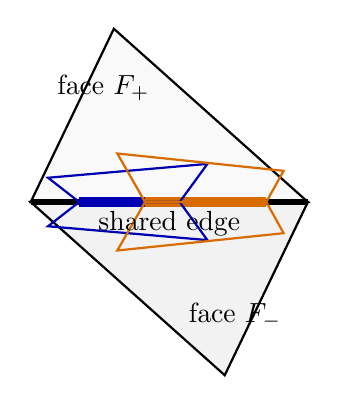
\begin{tikzpicture}[scale=.88]
  \coordinate (A) at (0,0); \coordinate (B) at (4,0);
  \coordinate (C) at (1.2,2.5); \coordinate (D) at (2.8,-2.5);
  \fill[gray!5] (A)--(B)--(C)--cycle;
  \fill[gray!10] (A)--(D)--(B)--cycle;
  \draw[thick] (A)--(B)--(C)--cycle;
  \draw[thick] (A)--(D)--(B)--cycle;
  \draw[line width=2.2pt] (A)--(B);
  \draw[blue!70!black,line width=3.5pt] (.7,0)--(2.15,0);
  \draw[orange!85!black,line width=3.5pt] (1.65,0)--(3.4,0);
  \draw[blue!70!black,thick] (.25,.35)--(.7,0)--(2.15,0)--(2.55,.55)--cycle;
  \draw[blue!70!black,thick] (.25,-.35)--(.7,0)--(2.15,0)--(2.55,-.55)--cycle;
  \draw[orange!85!black,thick] (1.25,.7)--(1.65,0)--(3.4,0)--(3.65,.45)--cycle;
  \draw[orange!85!black,thick] (1.25,-.7)--(1.65,0)--(3.4,0)--(3.65,-.45)--cycle;
  \node at (1.05,1.65) {face $F_+$};
  \node at (2.95,-1.65) {face $F_-$};
  \node[below] at (2,0) {shared edge};
\end{tikzpicture}

\caption{Two facewise polygonal models share the same strict membership
intervals on their common edge.  No equality of normal slopes is asserted.}
\label{fig:sharededge}
\end{figure}

The same observation gives a finite facewise statement.

\begin{proposition}[Finite facewise-compatible models]\label{prop:complex}
Let $K$ be a finite two-dimensional polyhedral complex whose facets are
convex polygons in their affine planes.  Suppose each facet carries a finite
open convex source realization, and the source traces agree on every shared
edge.  Then each facet admits a polygonal realization with the same face
code, and all incident realizations agree pointwise on every shared edge.
Protected face witnesses and finitely many additional line traces may be
retained.
\end{proposition}

\begin{proof}
Apply \cref{thm:main} independently to each facet, prescribing all of its
edge-supporting lines and the additional lines.  There are finitely many
facets.  Agreement on a shared edge follows from \cref{cor:sharededge}.
\end{proof}

\begin{remark}[No global convexity across the complex]
\Cref{prop:complex} is a coherent facewise output model.  It does not claim
that the union of the face pieces belonging to one neuron is convex in the
ambient space, or even that it is the trace of one higher-dimensional convex
set.
\end{remark}
